\documentclass[10pt]{IEEEtran}

\usepackage[utf8x]{inputenc}
\usepackage[L7x]{fontenc}
\usepackage[lithuanian]{babel}
\usepackage{listings}
\usepackage{epstopdf}

\lstset{
    basicstyle=\footnotesize,
    language=Java,
    morekeywords={String,each,in,Iterator}
}

\author{Maksim Norkin\\ \texttt{maksim.norkin@ieee.org}}
\title{Hadoop}

\begin{document}

    \maketitle

    \section{Laboratorinis darbas nr 1. Dalykinės srities pasirinkimas}

        \subsection{Užduotis}

            Dalykinę sritį aprašyti žodžiais ir pavaizduoti paveikslėlyje. Būtina bendrai aprašyti vykstančius verslo procesus. Ta pati pasirinktoji dalykinė sritis turi būti nagrinėjama visuose  tolimesniuose darbuose. 

            Reikia pateikti pasirinktos dalykinės srities aprašymą. Aprašymas turi būti tekstinis ir  iliustruotas vaizdžiuoju paveikslėliu. Aprašymui sudaryti turi būti naudojami dalykinės srities  terminai.Aprašymas turi atspindėti pagrindinius dalykinės srities aktorius, procesus bei įmonės veiklą įtakojančius išorinius agentus. Aiškiai turi būti išryškinta probleminė sritis, kuri parodo, kodėl yra svarbu nagrinėti pasirinktą dalykinę sritį. 

            Taip pat gali būti vaizduojami informaciniai srautai, materialiniai srautai, sistemos veiklą  kontroliuojantys elementai, dalyvių požiūriai ir emocijos, konfliktinės situacijos. Turi būti pateikta vaizdžiojo paveikslėlio specifikacija.

        \subsection{Įvadas}

            Dalykinė sritis pasirinkimas padaromas automobilių stovėjimą teikiančios įmonės naudai. Padarius šios srities analizę, nuspręsta, kad šioje srityje galima darbą optimizuoti galinio kliento naudai.

        \subsection{Analizė}

            Iškeliama problema yra randama kiekvienos dienos situacijoje, kuomet tik važiuojame į bet kokio pobūdžio susitikimą ir reikia automobilį palikti stovėjimo aikštelėje.

            \begin{figure}[t]
                \includegraphics{figures/struktura.eps}
                \label{fig:struktura}
                \caption{Dalykinės srities struktūra.}
            \end{figure}

        \subsection{Išvados}

    \section{Laboratorinis darbas nr. 2}

    \section{Laboratorinis darbas nr. 3}

    \section{Laboratorinis darbas nr. 4}

    \section{Laboratorinis darbas nr. 5}

\end{document}